% Options for packages loaded elsewhere
\PassOptionsToPackage{unicode}{hyperref}
\PassOptionsToPackage{hyphens}{url}
%
\documentclass[
]{book}
\usepackage{amsmath,amssymb}
\usepackage{lmodern}
\usepackage{ifxetex,ifluatex}
\ifnum 0\ifxetex 1\fi\ifluatex 1\fi=0 % if pdftex
  \usepackage[T1]{fontenc}
  \usepackage[utf8]{inputenc}
  \usepackage{textcomp} % provide euro and other symbols
\else % if luatex or xetex
  \usepackage{unicode-math}
  \defaultfontfeatures{Scale=MatchLowercase}
  \defaultfontfeatures[\rmfamily]{Ligatures=TeX,Scale=1}
\fi
% Use upquote if available, for straight quotes in verbatim environments
\IfFileExists{upquote.sty}{\usepackage{upquote}}{}
\IfFileExists{microtype.sty}{% use microtype if available
  \usepackage[]{microtype}
  \UseMicrotypeSet[protrusion]{basicmath} % disable protrusion for tt fonts
}{}
\makeatletter
\@ifundefined{KOMAClassName}{% if non-KOMA class
  \IfFileExists{parskip.sty}{%
    \usepackage{parskip}
  }{% else
    \setlength{\parindent}{0pt}
    \setlength{\parskip}{6pt plus 2pt minus 1pt}}
}{% if KOMA class
  \KOMAoptions{parskip=half}}
\makeatother
\usepackage{xcolor}
\IfFileExists{xurl.sty}{\usepackage{xurl}}{} % add URL line breaks if available
\IfFileExists{bookmark.sty}{\usepackage{bookmark}}{\usepackage{hyperref}}
\hypersetup{
  pdftitle={Introduction to Theoretical Ecology},
  pdfauthor={Instructor: Po-Ju Ke \textasciitilde\textasciitilde\textasciitilde\textasciitilde\textasciitilde{} Teaching Assistant: Gen-Chang Hsu},
  hidelinks,
  pdfcreator={LaTeX via pandoc}}
\urlstyle{same} % disable monospaced font for URLs
\usepackage{color}
\usepackage{fancyvrb}
\newcommand{\VerbBar}{|}
\newcommand{\VERB}{\Verb[commandchars=\\\{\}]}
\DefineVerbatimEnvironment{Highlighting}{Verbatim}{commandchars=\\\{\}}
% Add ',fontsize=\small' for more characters per line
\usepackage{framed}
\definecolor{shadecolor}{RGB}{248,248,248}
\newenvironment{Shaded}{\begin{snugshade}}{\end{snugshade}}
\newcommand{\AlertTok}[1]{\textcolor[rgb]{0.94,0.16,0.16}{#1}}
\newcommand{\AnnotationTok}[1]{\textcolor[rgb]{0.56,0.35,0.01}{\textbf{\textit{#1}}}}
\newcommand{\AttributeTok}[1]{\textcolor[rgb]{0.77,0.63,0.00}{#1}}
\newcommand{\BaseNTok}[1]{\textcolor[rgb]{0.00,0.00,0.81}{#1}}
\newcommand{\BuiltInTok}[1]{#1}
\newcommand{\CharTok}[1]{\textcolor[rgb]{0.31,0.60,0.02}{#1}}
\newcommand{\CommentTok}[1]{\textcolor[rgb]{0.56,0.35,0.01}{\textit{#1}}}
\newcommand{\CommentVarTok}[1]{\textcolor[rgb]{0.56,0.35,0.01}{\textbf{\textit{#1}}}}
\newcommand{\ConstantTok}[1]{\textcolor[rgb]{0.00,0.00,0.00}{#1}}
\newcommand{\ControlFlowTok}[1]{\textcolor[rgb]{0.13,0.29,0.53}{\textbf{#1}}}
\newcommand{\DataTypeTok}[1]{\textcolor[rgb]{0.13,0.29,0.53}{#1}}
\newcommand{\DecValTok}[1]{\textcolor[rgb]{0.00,0.00,0.81}{#1}}
\newcommand{\DocumentationTok}[1]{\textcolor[rgb]{0.56,0.35,0.01}{\textbf{\textit{#1}}}}
\newcommand{\ErrorTok}[1]{\textcolor[rgb]{0.64,0.00,0.00}{\textbf{#1}}}
\newcommand{\ExtensionTok}[1]{#1}
\newcommand{\FloatTok}[1]{\textcolor[rgb]{0.00,0.00,0.81}{#1}}
\newcommand{\FunctionTok}[1]{\textcolor[rgb]{0.00,0.00,0.00}{#1}}
\newcommand{\ImportTok}[1]{#1}
\newcommand{\InformationTok}[1]{\textcolor[rgb]{0.56,0.35,0.01}{\textbf{\textit{#1}}}}
\newcommand{\KeywordTok}[1]{\textcolor[rgb]{0.13,0.29,0.53}{\textbf{#1}}}
\newcommand{\NormalTok}[1]{#1}
\newcommand{\OperatorTok}[1]{\textcolor[rgb]{0.81,0.36,0.00}{\textbf{#1}}}
\newcommand{\OtherTok}[1]{\textcolor[rgb]{0.56,0.35,0.01}{#1}}
\newcommand{\PreprocessorTok}[1]{\textcolor[rgb]{0.56,0.35,0.01}{\textit{#1}}}
\newcommand{\RegionMarkerTok}[1]{#1}
\newcommand{\SpecialCharTok}[1]{\textcolor[rgb]{0.00,0.00,0.00}{#1}}
\newcommand{\SpecialStringTok}[1]{\textcolor[rgb]{0.31,0.60,0.02}{#1}}
\newcommand{\StringTok}[1]{\textcolor[rgb]{0.31,0.60,0.02}{#1}}
\newcommand{\VariableTok}[1]{\textcolor[rgb]{0.00,0.00,0.00}{#1}}
\newcommand{\VerbatimStringTok}[1]{\textcolor[rgb]{0.31,0.60,0.02}{#1}}
\newcommand{\WarningTok}[1]{\textcolor[rgb]{0.56,0.35,0.01}{\textbf{\textit{#1}}}}
\usepackage{longtable,booktabs,array}
\usepackage{calc} % for calculating minipage widths
% Correct order of tables after \paragraph or \subparagraph
\usepackage{etoolbox}
\makeatletter
\patchcmd\longtable{\par}{\if@noskipsec\mbox{}\fi\par}{}{}
\makeatother
% Allow footnotes in longtable head/foot
\IfFileExists{footnotehyper.sty}{\usepackage{footnotehyper}}{\usepackage{footnote}}
\makesavenoteenv{longtable}
\usepackage{graphicx}
\makeatletter
\def\maxwidth{\ifdim\Gin@nat@width>\linewidth\linewidth\else\Gin@nat@width\fi}
\def\maxheight{\ifdim\Gin@nat@height>\textheight\textheight\else\Gin@nat@height\fi}
\makeatother
% Scale images if necessary, so that they will not overflow the page
% margins by default, and it is still possible to overwrite the defaults
% using explicit options in \includegraphics[width, height, ...]{}
\setkeys{Gin}{width=\maxwidth,height=\maxheight,keepaspectratio}
% Set default figure placement to htbp
\makeatletter
\def\fps@figure{htbp}
\makeatother
\setlength{\emergencystretch}{3em} % prevent overfull lines
\providecommand{\tightlist}{%
  \setlength{\itemsep}{0pt}\setlength{\parskip}{0pt}}
\setcounter{secnumdepth}{5}
\usepackage{booktabs}
\usepackage{booktabs}
\usepackage{longtable}
\usepackage{array}
\usepackage{multirow}
\usepackage{wrapfig}
\usepackage{float}
\usepackage{colortbl}
\usepackage{pdflscape}
\usepackage{tabu}
\usepackage{threeparttable}
\usepackage{threeparttablex}
\usepackage[normalem]{ulem}
\usepackage{makecell}
\usepackage{xcolor}
\ifluatex
  \usepackage{selnolig}  % disable illegal ligatures
\fi
\usepackage[]{natbib}
\bibliographystyle{apalike}

\title{Introduction to Theoretical Ecology}
\author{Instructor: Po-Ju Ke \(~~~~~\) Teaching Assistant: Gen-Chang Hsu}
\date{2021 Fall at National Taiwan Univeristy \includegraphics{./bifurcation.gif}}

\begin{document}
\maketitle

{
\setcounter{tocdepth}{1}
\tableofcontents
}
\hypertarget{course-information}{%
\chapter*{Course Information}\label{course-information}}
\addcontentsline{toc}{chapter}{Course Information}

\textbf{IMPORTANT ANOUNCEMENT!!!}

The first three weeks of this course will be online. We will host the two modules of this course (i.e., 2-hr lecture and 1-hr practice) on different platforms. We will use Google Meet for the lecture section \href{https://meet.google.com/nzd-cdjp-kbt}{(link here)}. To mimic an environment where we can provide one-on-one coding advice, we will use Gather Town for the hands-on practice section \href{https://gather.town/app/osrqFSf0a7q0I6uo/TheoreticalEcology}{(link here)}. Please login in advance to make sure it is working; learn how to use Gather Town \href{https://www.youtube.com/watch?v=89at5EvCEvk}{here}.

For those who wish to enroll manually, please join the first lecture and stay online afterward. Since we have moved to a larger classroom due to COVID-19 regulation, we can accommodate more students. We have asked students to introduce themselves (e.g., research interest and familiarity with R; 1-2 minutes) during the first time we meet online, so please also be prepared if you wish to enroll.

\begin{center}\rule{0.5\linewidth}{0.5pt}\end{center}

\textbf{Description}

The development of theory plays an important role in advancing ecology as a scientific field. This three-unit course is for students at the graduate or advanced undergraduate level. The course will cover classic theoretical topics in ecology, starting from single-species dynamics and gradually build up to multi-species models. The course will primarily focus on population and community ecology, but we will also briefly discuss models in epidemiology and ecosystem ecology. Emphasis will be on theoretical concepts and corresponding mathematical approaches.

This course is designed as a two-hour lecture followed by a one-hour hands-on practice module. In the lecture, we will analyze dynamical models and derive general theories in ecology. In the hands-on practice section, we will use a combination of analytical problem sets, interactive applications, and numerical simulations to gain a general understanding of the dynamics and behavior of different models.

\textbf{Objectives}

By the end of the course, students are expected to be familiar with the basic building blocks of ecological models and would be able to formulate and analyze simple models of their own. The hands-on practice component should allow students to link their ecological intuition with the underlying mathematical model, helping them to better understand the primary literature of theoretical ecology.

\textbf{Requirements}

Students are expected to have a basic understanding of \textbf{Calculus} (e.g., freshman introductory course) and \textbf{Ecology}.

\textbf{Format}

Tuesday 1:20 pm \textasciitilde{} 4:20 pm at Classroom 3C, Life Science Building

\begin{itemize}
\tightlist
\item
  Lecture (two hours): selected topics of ecological theories and models (blackboard writing)
\item
  Lab (one hour): hands-on practice in programming and simulation (using R) + discussion
\end{itemize}

\textbf{Grading}

The final grade consists of:

\begin{enumerate}
\def\labelenumi{(\arabic{enumi})}
\tightlist
\item
  Assignment problem sets (60\%)
\item
  Midterm exam (15\%)
\item
  Final exam (15\%)
\item
  Course participation (10\%)
\end{enumerate}

\textbf{Course materials}

We will be using a combination of textbooks and literature articles on theoretical ecology in this course. Textbook chapters and additional reading materials will be provided (see \textbf{Syllabus} for more details).

Below are the textbook references:

\begin{itemize}
\tightlist
\item
  Case, Ted J. \emph{An illustrated guide to theoretical ecology}. Oxford University Press, 2000.
\item
  Gotelli, Nicholas J. \emph{A primer of ecology 4\textsuperscript{th} edition}. Sinauer Associates, 2008.
\item
  Pastor, John. \emph{Mathematical ecology of populations and ecosystems}. John Wiley \& Sons, 2011.
\item
  Otto, Sarah P. and Troy Day. \emph{A biologist's guide to mathematical modeling in ecology and evolution}. Princeton University Press, 2011.
\end{itemize}

\textbf{Contacts}

\textbf{Instructor}: Po-Ju Ke

\begin{itemize}
\tightlist
\item
  Office: Life Science Building R635
\item
  Email: \href{mailto:pojuke@ntu.edu.tw}{\nolinkurl{pojuke@ntu.edu.tw}}
\item
  Office hours: by appointment
\end{itemize}

\textbf{Teaching assistant}: Gen-Chang Hsu

\begin{itemize}
\tightlist
\item
  Email: \href{mailto:b04b01065@ntu.edu.tw}{\nolinkurl{b04b01065@ntu.edu.tw}}
\item
  Office hours: by appointment
\end{itemize}

\hypertarget{syllabus}{%
\chapter*{Syllabus}\label{syllabus}}
\addcontentsline{toc}{chapter}{Syllabus}

\begingroup\fontsize{17}{19}\selectfont

\begin{tabu} to \linewidth {>{\centering}X>{\centering}X>{\centering}X>{\raggedright}X}
\hline
\begingroup\fontsize{20}{22}\selectfont \textcolor{black}{\textbf{Date}}\endgroup & \begingroup\fontsize{20}{22}\selectfont \textcolor{black}{\textbf{Lecture topic}}\endgroup & \begingroup\fontsize{20}{22}\selectfont \textcolor{black}{\textbf{Lab}}\endgroup & \begingroup\fontsize{20}{22}\selectfont \textcolor{black}{\textbf{Readings}}\endgroup\\
\hline
**Week 1** <span style='vertical-align:-30%'> </span>
           <br> 28-Sept-2021 & Introduction: what is theoretical ecology? & \- & Grainger et al., 2021\\
\hline
**Week 2** <span style='vertical-align:-30%'> </span>
           <br> 05-Oct-2021 & Exponential population growth & Solving exponential growth equation using "deSolve" & Visualization & Gotelli [Ch.1] <br> Case [Ch.1]\\
\hline
**Week 3** <span style='vertical-align:-30%'> </span>
           <br> 12-Oct-2021 & Logistic population growth and stability analysis & Solving logistic growth equation using "deSolve" & Visualization & Gotelli [Ch.2] <br> Case [Ch.5] <br> Otto & Day [Ch.5]\\
\hline
**Week 4** <span style='vertical-align:-30%'> </span>
           <br> 19-Oct-2021 & Discrete exponential and logistic models &  & May, 1976\\
\hline
**Week 5** <span style='vertical-align:-30%'> </span>
           <br> 26-Oct-2021 & Age-structured models & Analyzing Leslie matrix using for loops and eigenanalysis & Gotelli [Ch.3] <br> Case[Ch.3]\\
\hline
**Week 6** <span style='vertical-align:-30%'> </span>
           <br> 02-Nov-2021 & Metapopulations and patch occupancy models &  & Gotelli [Ch.4] <br> Case [Ch.16]\\
\hline
**Week 7** <span style='vertical-align:-30%'> </span>
           <br> 09-Nov-2021 & Lotka-Volterra model of competition: graphical analysis &  & Gotelli [Ch.5] <br> Case [Ch.14]\\
\hline
**Week 8** <span style='vertical-align:-30%'> </span>
           <br> 16-Nov-2021 & Lotka-Volterra model of competition: linear stability analysis &  & Otto & Day [Ch.8]\\
\hline
**Week 9** <span style='vertical-align:-30%'> </span>
           <br> 23-Nov-2021 & Midterm exam & \- & $~~~~~~~~~~~~$ \-\\
\hline
**Week 10** <span style='vertical-align:-30%'> </span>
           <br> 30-Nov-2021 & Predator-prey interactions &  & Gotelli [Ch.6] <br> Case [Ch.12 & 13]\\
\hline
**Week 11** <span style='vertical-align:-30%'> </span>
           <br> 07-Dec-2021 & Mutualisms &  & Vandermeer & Boucher, 1978\\
\hline
**Week 12** <span style='vertical-align:-30%'> </span>
           <br> 14-Dec-2021 & Multispecies models of competition: apparent and exploitative competition &  & Holt, 1977.\\
\hline
**Week 13** <span style='vertical-align:-30%'> </span>
           <br> 21-Dec-2021 & Multispecies models of predation: food chains and intraguild predation &  & Holt & Polis, 1997\\
\hline
**Week 14** <span style='vertical-align:-30%'> </span>
           <br> 28-Dec-2021 & Disease dynamics and SIR models &  & Anderson & May, 1979\\
\hline
**Week 15** <span style='vertical-align:-30%'> </span>
           <br> 04-Jan-2022 & Ecosystem models and feedbacks &  & Pastor [Ch.11 & 12]\\
\hline
**Week 16** <span style='vertical-align:-30%'> </span>
           <br> 11-Jan-2022 & Final exam & \- & $~~~~~~~~~~~~$ \-\\
\hline
\end{tabu}
\endgroup{}

\hypertarget{week-1}{%
\chapter*{Week 1}\label{week-1}}
\addcontentsline{toc}{chapter}{Week 1}

\textbf{\emph{Introduction: what is theoretical ecology?}}

\hypertarget{lecture-in-a-nutshell}{%
\section*{Lecture in a nutshell}\label{lecture-in-a-nutshell}}
\addcontentsline{toc}{section}{Lecture in a nutshell}

\href{./Lecture\%20handouts/Week1_Lecture_What_Is_Theoretical_Ecology.pdf}{Lecture handout}

\begin{itemize}
\item
  Introduction to ecological theories and mathematical models
\item
  Constructing ecological models: 5 steps
\end{itemize}

{\textbf{\emph{Step 1}}. Formulate the motivating question}

{\textbf{\emph{Step 2}}. Determine the basic ingredients}

{\textbf{\emph{Step 3}}. Qualitatively describe the biological system}

{\textbf{\emph{Step 4}}. Quantitatively describe the biological system}

{\textbf{\emph{Step 5}}. Analyze the model}

\begin{itemize}
\tightlist
\item
  Apply ecological models in your study: 4 approaches
\end{itemize}

{\textbf{\emph{Approach 1}}. Adopt the framework}

{\textbf{\emph{Approach 2}}. Test the predictions}

{\textbf{\emph{Approach 3}}. Use the equations (model fitting/proxy calculation)}

{\textbf{\emph{Approach 4}}. Test model assumptions}

\begin{itemize}
\tightlist
\item
  Some relevant math techniques: Derivatives and integrals, linear approximation and Taylor expansion
\end{itemize}

\hypertarget{lab-demonstration}{%
\section*{Lab demonstration}\label{lab-demonstration}}
\addcontentsline{toc}{section}{Lab demonstration}

No lab demonstration this week.

\hypertarget{additional-readings}{%
\section*{Additional readings}\label{additional-readings}}
\addcontentsline{toc}{section}{Additional readings}

\href{./Additional\%20readings/Grainger_et_al_2021_AmNat.pdf}{Grainger et al.~(2021). An empiricist's guide to using ecological theory. \emph{American Naturalist}.}

\hypertarget{assignments}{%
\section*{Assignments}\label{assignments}}
\addcontentsline{toc}{section}{Assignments}

Please review the study material and make sure you understand the basic R syntax and programming fundamentals, which we will be using throughout the semester. The example dataset for the tutorial is provided below.

\href{./Assignments/Week1_Basic\%20Introduction\%20to\%20R.pdf}{Basic Introduction to R}

\href{./Assignments/example_dat.txt}{Example dataset}

\hypertarget{week-2}{%
\chapter*{Week 2}\label{week-2}}
\addcontentsline{toc}{chapter}{Week 2}

\textbf{\emph{Exponential population growth}}

\hypertarget{lecture-in-a-nutshell-1}{%
\section*{Lecture in a nutshell}\label{lecture-in-a-nutshell-1}}
\addcontentsline{toc}{section}{Lecture in a nutshell}

\begin{itemize}
\tightlist
\item
  \textbf{Model derivation:}

  \begin{enumerate}
  \def\labelenumi{\arabic{enumi}.}
  \tightlist
  \item
    Population growth rate: \(Birth - Death + Immigration - Emigration\)
  \item
    Per capita growth rate: \((birth - death + immigration - emigration)\times N\).
  \end{enumerate}
\end{itemize}

\begin{itemize}
\tightlist
\item
  \textbf{Assumptions:}

  \begin{enumerate}
  \def\labelenumi{\arabic{enumi}.}
  \tightlist
  \item
    Closed population: \(Immigration\) = \(Emigration = 0\)
  \item
    All individuals are identical: no genetic/age/stage structure
  \item
    Continuous population growth: no time lag
  \item
    Per capita birth and death rates are constant: time- and density-independent
  \end{enumerate}
\end{itemize}

\begin{itemize}
\tightlist
\item
  \textbf{Solving the differential equation \(\frac{dN}{dt} = (b-d)N\):}

  \begin{enumerate}
  \def\labelenumi{\arabic{enumi}.}
  \tightlist
  \item
    Use separation of variables and integrate both sides
  \item
    Plug in the initial condition \(N_0\) at \(t = 0\)
  \item
    Integration result: \(N_{(t)} = N_0e^{(b-d)t} = N_0e^{rt}\)
  \end{enumerate}
\end{itemize}

\begin{itemize}
\tightlist
\item
  \textbf{Related concept:}

  \begin{enumerate}
  \def\labelenumi{\arabic{enumi}.}
  \tightlist
  \item
    Doubling time \(t_d = \frac{ln(2)}{r}\)
  \end{enumerate}
\end{itemize}

\begin{itemize}
\tightlist
\item
  \textbf{Average (expected) lifetime for an exponential decay function \(N_{(t)} = N_0e^{-\delta t}\):}

  \begin{enumerate}
  \def\labelenumi{\arabic{enumi}.}
  \tightlist
  \item
    Probability density function (PDF): \(\frac{N_0e^{-\delta t} - N_0e^{-\delta (t+\Delta t)}}{N_0} \approx \delta e^{-\delta t}\) (linear approximation)
  \item
    Expected value: \(\int_{0}^{\infty}t\delta e^{-\delta t}dt\)
  \item
    Use integration by parts to evaluate the integral
  \item
    Integration result: \(\frac{1}{\delta}\)
  \end{enumerate}
\end{itemize}

\begin{itemize}
\tightlist
\item
  \textbf{Relaxation of assumption 1:}

  \begin{enumerate}
  \def\labelenumi{\arabic{enumi}.}
  \tightlist
  \item
    Net immigration/emigration is not zero: \(\frac{dN}{dt} = rN + I_{(t)}\)
  \item
    Solve the equation using the general solution to first-order linear differential equations
  \end{enumerate}
\end{itemize}

\begin{itemize}
\tightlist
\item
  \textbf{Relaxation of assumption 4:}

  \begin{enumerate}
  \def\labelenumi{\arabic{enumi}.}
  \tightlist
  \item
    Per capita growth rate \(r\) is not a constant but rather a function of time: \(\frac{dN}{dt} = r_{(t)}N\)
  \item
    An example of \(r_{(t)}\): \(r_{(t)} = \overline{r} + \frac{\sigma}{2}sin(\omega t + \phi)\)
  \item
    Biological interpretation of \(r_{(t)}\): seasonality, environmental fluctuations, etc.
  \end{enumerate}
\end{itemize}

\hypertarget{lab-demonstration-1}{%
\section*{Lab demonstration}\label{lab-demonstration-1}}
\addcontentsline{toc}{section}{Lab demonstration}

In this lab, we will be solving the differential equation for exponential population growth (Part 1) and visualize how the population sizes change over time (Part 2).

\textbf{Part 1 - Numerical solution using the package ``deSolve''}

Two main phases:

\protect\hypertarget{aaa}{}{Model specification: specify the structure of differential equation model}

\protect\hypertarget{bbb}{}{Model application: set the time steps, initial population size, model parameters (e.g., intrinsic population growth rate \emph{r}) and solve the equation}

\begin{Shaded}
\begin{Highlighting}[]
\CommentTok{\# install.packages("deSolve")}
\FunctionTok{library}\NormalTok{(deSolve)}

\DocumentationTok{\#\#\# (1) Model specification}
\NormalTok{exponential\_model }\OtherTok{\textless{}{-}} \ControlFlowTok{function}\NormalTok{(times, state, parms) \{}
  \FunctionTok{with}\NormalTok{(}\FunctionTok{as.list}\NormalTok{(}\FunctionTok{c}\NormalTok{(state, parms)), \{}
\NormalTok{    dN\_dt }\OtherTok{=}\NormalTok{ r}\SpecialCharTok{*}\NormalTok{N  }\CommentTok{\# exponential growth equation}
    \FunctionTok{return}\NormalTok{(}\FunctionTok{list}\NormalTok{(}\FunctionTok{c}\NormalTok{(dN\_dt)))  }\CommentTok{\# return the results  }
\NormalTok{  \})}
\NormalTok{\}}

\DocumentationTok{\#\#\# (2) Model application}
\NormalTok{times }\OtherTok{\textless{}{-}} \FunctionTok{seq}\NormalTok{(}\DecValTok{0}\NormalTok{, }\DecValTok{10}\NormalTok{, }\AttributeTok{by =} \FloatTok{0.1}\NormalTok{)  }\CommentTok{\# time steps to integrate over}
\NormalTok{state }\OtherTok{\textless{}{-}} \FunctionTok{c}\NormalTok{(}\AttributeTok{N =} \DecValTok{10}\NormalTok{)  }\CommentTok{\# initial population size}
\NormalTok{parms }\OtherTok{\textless{}{-}} \FunctionTok{c}\NormalTok{(}\AttributeTok{r =} \FloatTok{1.5}\NormalTok{)  }\CommentTok{\# intrinsic growth rate}

\CommentTok{\# run the ode solver}
\NormalTok{pop\_size }\OtherTok{\textless{}{-}} \FunctionTok{ode}\NormalTok{(}\AttributeTok{func =}\NormalTok{ exponential\_model, }\AttributeTok{times =}\NormalTok{ times, }\AttributeTok{y =}\NormalTok{ state, }\AttributeTok{parms =}\NormalTok{ parms)}

\CommentTok{\# take a look at the results}
\FunctionTok{head}\NormalTok{(pop\_size)}
\end{Highlighting}
\end{Shaded}

\begin{verbatim}
##      time        N
## [1,]  0.0 10.00000
## [2,]  0.1 11.61834
## [3,]  0.2 13.49860
## [4,]  0.3 15.68313
## [5,]  0.4 18.22120
## [6,]  0.5 21.17002
\end{verbatim}

\textbf{Part 2. Visualize the integration results:}

Linear scale

\begin{Shaded}
\begin{Highlighting}[]
\CommentTok{\# install.packages("tidyverse")}
\FunctionTok{library}\NormalTok{(tidyverse)}

\FunctionTok{ggplot}\NormalTok{(}\AttributeTok{data =} \FunctionTok{as.data.frame}\NormalTok{(pop\_size), }\FunctionTok{aes}\NormalTok{(}\AttributeTok{x =}\NormalTok{ time, }\AttributeTok{y =}\NormalTok{ N)) }\SpecialCharTok{+} 
  \FunctionTok{geom\_point}\NormalTok{() }\SpecialCharTok{+} 
  \FunctionTok{labs}\NormalTok{(}\AttributeTok{title =} \FunctionTok{paste0}\NormalTok{(}\StringTok{"Exponential Growth }\SpecialCharTok{\textbackslash{}n}\StringTok{ (r = "}\NormalTok{, parms[}\StringTok{"r"}\NormalTok{], }\StringTok{")"}\NormalTok{)) }\SpecialCharTok{+}
  \FunctionTok{theme\_classic}\NormalTok{(}\AttributeTok{base\_size =} \DecValTok{12}\NormalTok{) }\SpecialCharTok{+} 
  \FunctionTok{theme}\NormalTok{(}\AttributeTok{plot.title =} \FunctionTok{element\_text}\NormalTok{(}\AttributeTok{hjust =} \FloatTok{0.5}\NormalTok{)) }\SpecialCharTok{+}
  \FunctionTok{scale\_x\_continuous}\NormalTok{(}\AttributeTok{limits =} \FunctionTok{c}\NormalTok{(}\DecValTok{0}\NormalTok{, }\FloatTok{10.5}\NormalTok{), }\AttributeTok{expand =} \FunctionTok{c}\NormalTok{(}\DecValTok{0}\NormalTok{, }\DecValTok{0}\NormalTok{)) }\SpecialCharTok{+}
  \FunctionTok{scale\_y\_continuous}\NormalTok{(}\AttributeTok{limits =} \FunctionTok{c}\NormalTok{(}\DecValTok{0}\NormalTok{, }\FunctionTok{max}\NormalTok{(}\FunctionTok{as.data.frame}\NormalTok{(pop\_size)}\SpecialCharTok{$}\NormalTok{N)}\SpecialCharTok{*}\FloatTok{1.1}\NormalTok{), }\AttributeTok{expand =} \FunctionTok{c}\NormalTok{(}\DecValTok{0}\NormalTok{, }\DecValTok{0}\NormalTok{))}
\end{Highlighting}
\end{Shaded}

\begin{center}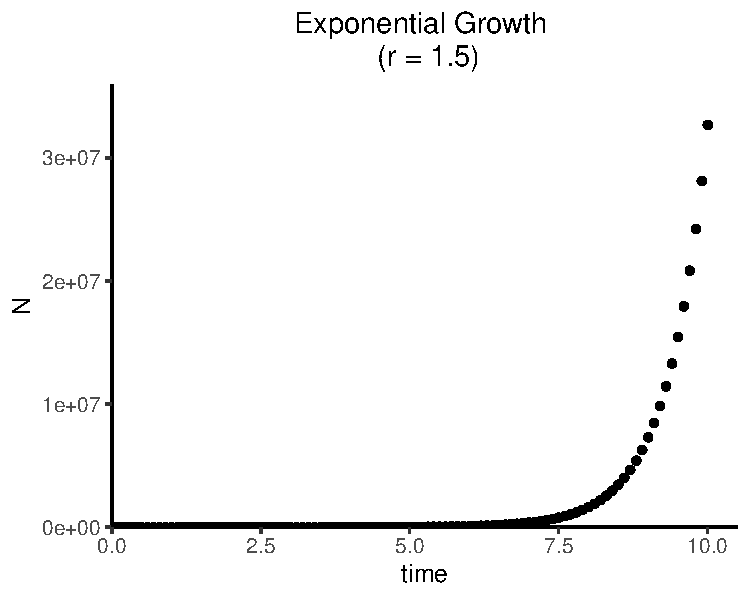
\includegraphics[width=0.7\linewidth]{02_Week_2_files/figure-latex/unnamed-chunk-2-1} \end{center}

Log scale

\begin{Shaded}
\begin{Highlighting}[]
\FunctionTok{ggplot}\NormalTok{(}\AttributeTok{data =} \FunctionTok{as.data.frame}\NormalTok{(pop\_size), }\FunctionTok{aes}\NormalTok{(}\AttributeTok{x =}\NormalTok{ time, }\AttributeTok{y =}\NormalTok{ N)) }\SpecialCharTok{+} 
  \FunctionTok{geom\_point}\NormalTok{() }\SpecialCharTok{+} 
  \FunctionTok{labs}\NormalTok{(}\AttributeTok{title =} \FunctionTok{paste0}\NormalTok{(}\StringTok{"Exponential Growth }\SpecialCharTok{\textbackslash{}n}\StringTok{ (r = "}\NormalTok{, parms[}\StringTok{"r"}\NormalTok{], }\StringTok{")"}\NormalTok{)) }\SpecialCharTok{+}
  \FunctionTok{theme\_classic}\NormalTok{(}\AttributeTok{base\_size =} \DecValTok{12}\NormalTok{) }\SpecialCharTok{+} 
  \FunctionTok{theme}\NormalTok{(}\AttributeTok{plot.title =} \FunctionTok{element\_text}\NormalTok{(}\AttributeTok{hjust =} \FloatTok{0.5}\NormalTok{)) }\SpecialCharTok{+} 
  \FunctionTok{scale\_x\_continuous}\NormalTok{(}\AttributeTok{limits =} \FunctionTok{c}\NormalTok{(}\DecValTok{0}\NormalTok{, }\FloatTok{10.5}\NormalTok{), }\AttributeTok{expand =} \FunctionTok{c}\NormalTok{(}\DecValTok{0}\NormalTok{, }\DecValTok{0}\NormalTok{)) }\SpecialCharTok{+}
  \FunctionTok{scale\_y\_log10}\NormalTok{(}\AttributeTok{breaks =}\NormalTok{ scales}\SpecialCharTok{::}\FunctionTok{trans\_breaks}\NormalTok{(}\StringTok{"log10"}\NormalTok{, }\ControlFlowTok{function}\NormalTok{(x) }\DecValTok{10}\SpecialCharTok{\^{}}\NormalTok{x)(}\FunctionTok{c}\NormalTok{(}\DecValTok{10}\NormalTok{, }\DecValTok{10}\SpecialCharTok{\^{}}\DecValTok{7}\NormalTok{)),}
                \AttributeTok{labels =}\NormalTok{ scales}\SpecialCharTok{::}\FunctionTok{trans\_format}\NormalTok{(}\StringTok{"log10"}\NormalTok{, scales}\SpecialCharTok{::}\FunctionTok{math\_format}\NormalTok{(}\DecValTok{10}\SpecialCharTok{\^{}}\NormalTok{.x)),}
                \AttributeTok{expand =} \FunctionTok{c}\NormalTok{(}\DecValTok{0}\NormalTok{, }\DecValTok{0}\NormalTok{))}
\end{Highlighting}
\end{Shaded}

\begin{center}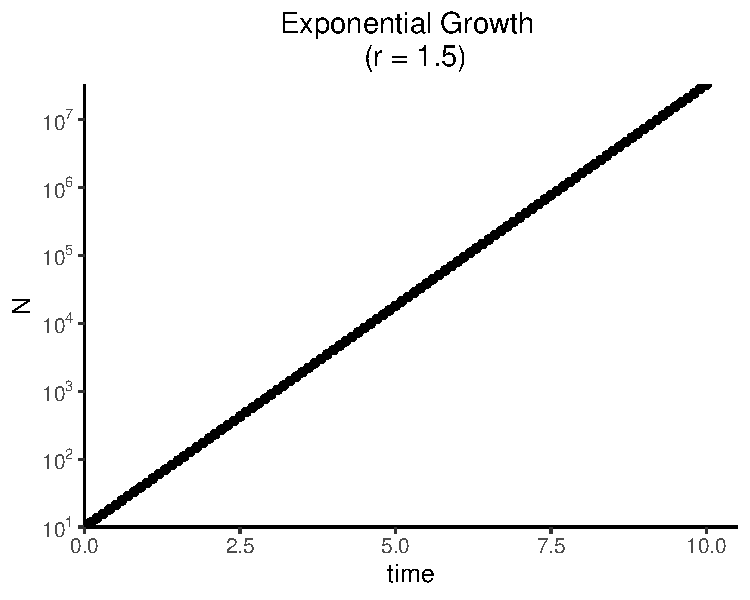
\includegraphics[width=0.7\linewidth]{02_Week_2_files/figure-latex/unnamed-chunk-3-1} \end{center}

\hypertarget{additional-readings-1}{%
\section*{Additional readings}\label{additional-readings-1}}
\addcontentsline{toc}{section}{Additional readings}

\href{./Additional\%20readings/Package\%20deSolve\%20-\%20Solving\%20Initial\%20Value\%20Differential\%20Equations\%20in\%20R.pdf}{Package deSolve: Solving Initial Value Differential Equations in R}

\hypertarget{assignments-1}{%
\section*{Assignments}\label{assignments-1}}
\addcontentsline{toc}{section}{Assignments}

\href{./Assignments/Week2_Exponential\%20Growth.pdf}{Exponential Population Growth with Constant Immigration}

\hypertarget{week-3}{%
\chapter*{Week 3}\label{week-3}}
\addcontentsline{toc}{chapter}{Week 3}

\textbf{\emph{Logistic population growth and stability analysis}}

\hypertarget{lecture-in-a-nutshell-2}{%
\section*{Lecture in a nutshell}\label{lecture-in-a-nutshell-2}}
\addcontentsline{toc}{section}{Lecture in a nutshell}

\hypertarget{lab-demonstration-2}{%
\section*{Lab demonstration}\label{lab-demonstration-2}}
\addcontentsline{toc}{section}{Lab demonstration}

In this lab, we will solve the differential equation for logistic population growth and visualize how the population sizes change over time. Have a quick review of the \href{https://genchanghsu.github.io/2021_Fall_Introduction_to_Theoretical_Ecology/week-2.html\#lab-demonstration-1}{lab section} in Week 2.

We will also take a look at how population growth rate (\(\frac{dN}{dt}\)) and per capita growth rate (\(\frac{dN}{dtN}\)) change with population size (\(N\)).

\textbf{Part 1 - Solving the logistic growth equation and visualize the results}

Here is an interactive web app for the logistic growth model. Feel free to play around with the parameters/values and see how the population trajectories change.

Please select a set of parameters of your choice and reproduce the output figure you see in this app (hint: you can modify the code in Week 2).

\href{https://genchanghsu0115.shinyapps.io/Logistic_mod_shinyapp/}{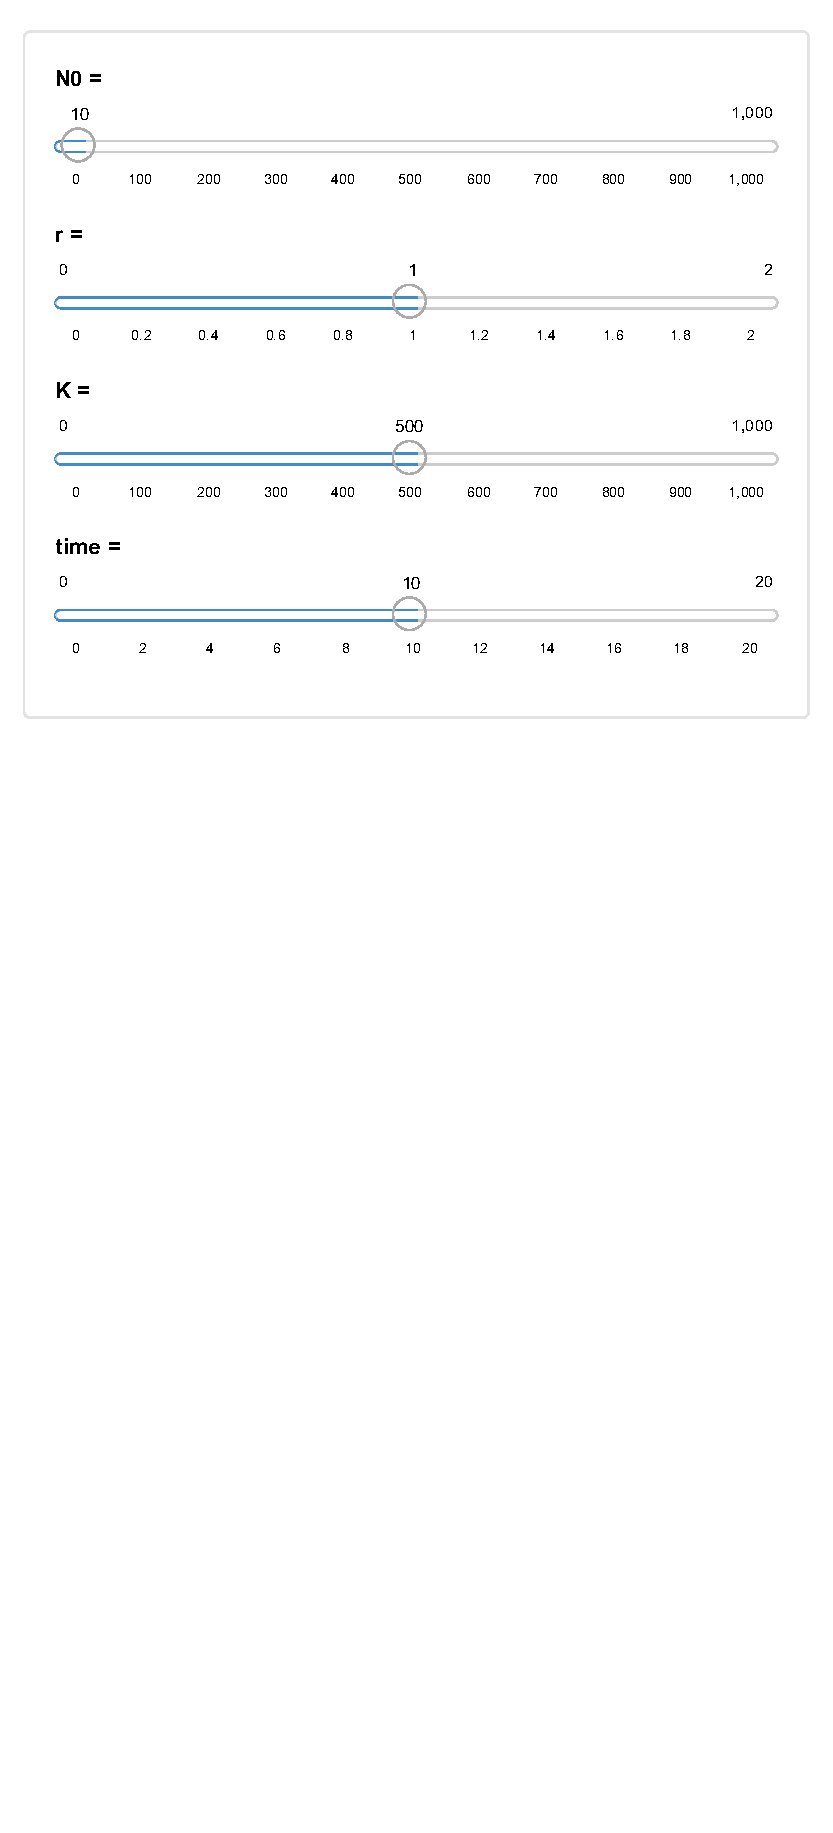
\includegraphics[width=800px]{03_Week_3_files/figure-latex/unnamed-chunk-2-1} }

\textbf{Part 2 - The relationship between population growth rate (\(\frac{dN}{dt}\))/per capita growth rate (\(\frac{dN}{dtN}\)) and population size (\(N\))}

\begin{Shaded}
\begin{Highlighting}[]
\CommentTok{\# parameters}
\NormalTok{r }\OtherTok{\textless{}{-}} \FloatTok{1.5}
\NormalTok{K }\OtherTok{\textless{}{-}} \DecValTok{500}

\CommentTok{\# a vector of population sizes}
\NormalTok{N }\OtherTok{\textless{}{-}} \DecValTok{0}\SpecialCharTok{:}\DecValTok{600}

\CommentTok{\# calculate the population growth rates and per capita growth rates}
\NormalTok{dN\_dt }\OtherTok{\textless{}{-}}\NormalTok{ r}\SpecialCharTok{*}\NormalTok{N}\SpecialCharTok{*}\NormalTok{(K}\SpecialCharTok{{-}}\NormalTok{N)}\SpecialCharTok{/}\NormalTok{K }
\NormalTok{dN\_dtN }\OtherTok{\textless{}{-}}\NormalTok{ r}\SpecialCharTok{*}\NormalTok{(K}\SpecialCharTok{{-}}\NormalTok{N)}\SpecialCharTok{/}\NormalTok{K}

\CommentTok{\# organize into a dataframe}
\NormalTok{logistic\_data }\OtherTok{\textless{}{-}} \FunctionTok{data.frame}\NormalTok{(N, dN\_dt, dN\_dtN) }\SpecialCharTok{\%\textgreater{}\%}
  \FunctionTok{pivot\_longer}\NormalTok{(}\AttributeTok{cols =} \FunctionTok{c}\NormalTok{(dN\_dt, dN\_dtN), }
               \AttributeTok{names\_to =} \StringTok{"vars"}\NormalTok{, }
               \AttributeTok{values\_to =} \StringTok{"values"}\NormalTok{)}

\CommentTok{\# plot }
\NormalTok{K\_df }\OtherTok{\textless{}{-}} \FunctionTok{data.frame}\NormalTok{(}\AttributeTok{xend =} \FunctionTok{c}\NormalTok{(}\DecValTok{500}\NormalTok{, }\DecValTok{500}\NormalTok{),}
                   \AttributeTok{yend =} \FunctionTok{c}\NormalTok{(}\DecValTok{20}\NormalTok{, }\FloatTok{0.1}\NormalTok{),}
                   \AttributeTok{xstart =} \FunctionTok{c}\NormalTok{(}\DecValTok{500}\NormalTok{, }\DecValTok{500}\NormalTok{),}
                   \AttributeTok{ystart =} \FunctionTok{c}\NormalTok{(}\DecValTok{100}\NormalTok{, }\FloatTok{0.5}\NormalTok{),}
                   \AttributeTok{labels =} \FunctionTok{c}\NormalTok{(}\StringTok{"italic(K)"}\NormalTok{, }\StringTok{"italic(K)"}\NormalTok{),}
                   \AttributeTok{vars =} \FunctionTok{c}\NormalTok{(}\StringTok{"dN\_dt"}\NormalTok{, }\StringTok{"dN\_dtN"}\NormalTok{))}

\FunctionTok{ggplot}\NormalTok{(}\AttributeTok{data =}\NormalTok{ logistic\_data, }\FunctionTok{aes}\NormalTok{(}\AttributeTok{x =}\NormalTok{ N, }\AttributeTok{y =}\NormalTok{ values)) }\SpecialCharTok{+} 
  \FunctionTok{geom\_line}\NormalTok{(}\AttributeTok{size =} \FloatTok{1.2}\NormalTok{) }\SpecialCharTok{+} 
  \FunctionTok{geom\_point}\NormalTok{(}\AttributeTok{x =} \DecValTok{500}\NormalTok{, }\AttributeTok{y =} \DecValTok{0}\NormalTok{, }\AttributeTok{size =} \DecValTok{4}\NormalTok{, }\AttributeTok{color =} \StringTok{"blue"}\NormalTok{) }\SpecialCharTok{+}
  \FunctionTok{geom\_hline}\NormalTok{(}\AttributeTok{yintercept =} \DecValTok{0}\NormalTok{, }\AttributeTok{linetype =} \StringTok{"dashed"}\NormalTok{, }\AttributeTok{color =} \StringTok{"red"}\NormalTok{, }\AttributeTok{size =} \FloatTok{1.2}\NormalTok{) }\SpecialCharTok{+}
  \FunctionTok{labs}\NormalTok{(}\AttributeTok{x =} \StringTok{"N"}\NormalTok{, }\AttributeTok{y =} \StringTok{""}\NormalTok{) }\SpecialCharTok{+}
  \FunctionTok{facet\_wrap}\NormalTok{(}\SpecialCharTok{\textasciitilde{}}\NormalTok{vars, }
             \AttributeTok{ncol =} \DecValTok{2}\NormalTok{, }
             \AttributeTok{scales =} \StringTok{"free\_y"}\NormalTok{,}
             \AttributeTok{strip.position =} \StringTok{"left"}\NormalTok{, }
             \AttributeTok{labeller =} \FunctionTok{as\_labeller}\NormalTok{(}\FunctionTok{c}\NormalTok{(}\AttributeTok{dN\_dt =} \StringTok{"dN/dt"}\NormalTok{, }
                                      \AttributeTok{dN\_dtN =} \StringTok{"dN/dtN"}\NormalTok{))) }\SpecialCharTok{+} 
  \FunctionTok{theme\_bw}\NormalTok{(}\AttributeTok{base\_size =} \DecValTok{12}\NormalTok{) }\SpecialCharTok{+}
  \FunctionTok{theme}\NormalTok{(}\AttributeTok{strip.background =} \FunctionTok{element\_blank}\NormalTok{(),}
        \AttributeTok{strip.placement =} \StringTok{"outside"}\NormalTok{,}
        \AttributeTok{legend.position =} \StringTok{"top"}\NormalTok{,}
        \AttributeTok{legend.title =} \FunctionTok{element\_blank}\NormalTok{()) }\SpecialCharTok{+} 
  \FunctionTok{scale\_x\_continuous}\NormalTok{(}\AttributeTok{limits =} \FunctionTok{c}\NormalTok{(}\DecValTok{0}\NormalTok{, }\DecValTok{610}\NormalTok{), }\AttributeTok{expand =} \FunctionTok{c}\NormalTok{(}\DecValTok{0}\NormalTok{, }\DecValTok{0}\NormalTok{)) }\SpecialCharTok{+} 
  \FunctionTok{geom\_segment}\NormalTok{(}\AttributeTok{data =}\NormalTok{ K\_df, }
               \FunctionTok{aes}\NormalTok{(}\AttributeTok{x =}\NormalTok{ xstart, }\AttributeTok{y =}\NormalTok{ ystart, }\AttributeTok{xend =}\NormalTok{ xend, }\AttributeTok{yend =}\NormalTok{ yend), }
               \AttributeTok{arrow =} \FunctionTok{arrow}\NormalTok{(}\AttributeTok{length =} \FunctionTok{unit}\NormalTok{(}\FloatTok{0.03}\NormalTok{, }\StringTok{"npc"}\NormalTok{)), }
               \AttributeTok{size =} \FloatTok{1.2}\NormalTok{,}
               \AttributeTok{color =} \StringTok{"blue"}\NormalTok{) }\SpecialCharTok{+} 
  \FunctionTok{geom\_text}\NormalTok{(}\AttributeTok{data =}\NormalTok{ K\_df, }
            \FunctionTok{aes}\NormalTok{(}\AttributeTok{x =}\NormalTok{ xstart, }\AttributeTok{y =}\NormalTok{ ystart}\SpecialCharTok{*}\FloatTok{1.2}\NormalTok{, }\AttributeTok{label =}\NormalTok{ labels),}
            \AttributeTok{size =} \DecValTok{5}\NormalTok{, }
            \AttributeTok{color =} \StringTok{"blue"}\NormalTok{,}
            \AttributeTok{parse =}\NormalTok{ T)}
\end{Highlighting}
\end{Shaded}

\begin{center}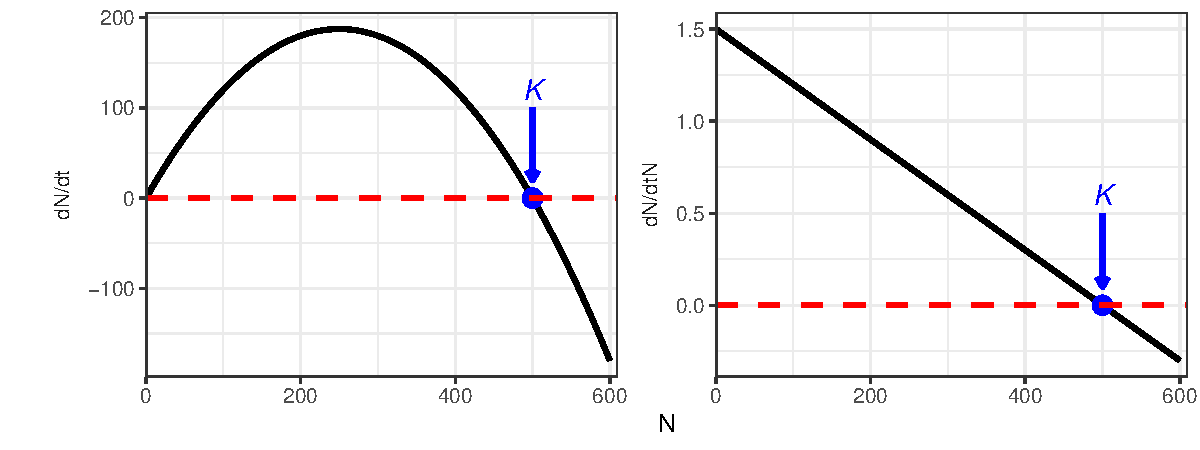
\includegraphics[width=0.95\linewidth]{03_Week_3_files/figure-latex/unnamed-chunk-3-1} \end{center}

\hypertarget{additional-readings-2}{%
\section*{Additional readings}\label{additional-readings-2}}
\addcontentsline{toc}{section}{Additional readings}

\href{http://equation-of-the-month.blogspot.com/2012/01/logistic-growth.html}{Logistic Growth}

\hypertarget{assignments-2}{%
\section*{Assignments}\label{assignments-2}}
\addcontentsline{toc}{section}{Assignments}

\href{./Assignments/Week3_Logistic\%20Growth.pdf}{Population Growth with Allee Effects}

\hypertarget{week-4}{%
\chapter*{Week 4}\label{week-4}}
\addcontentsline{toc}{chapter}{Week 4}

\textbf{\emph{Discrete exponential and logistic models}}

\hypertarget{lecture-in-a-nutshell-3}{%
\section*{Lecture in a nutshell}\label{lecture-in-a-nutshell-3}}
\addcontentsline{toc}{section}{Lecture in a nutshell}

\hypertarget{lab-demonstration-3}{%
\section*{Lab demonstration}\label{lab-demonstration-3}}
\addcontentsline{toc}{section}{Lab demonstration}

\hypertarget{additional-readings-3}{%
\section*{Additional readings}\label{additional-readings-3}}
\addcontentsline{toc}{section}{Additional readings}

\href{./Additional\%20readings/May_1976_Nature.pdf}{Simple mathematical models with very complicated dynamics}

\hypertarget{assignments-3}{%
\section*{Assignments}\label{assignments-3}}
\addcontentsline{toc}{section}{Assignments}

\hypertarget{week-5}{%
\chapter*{Week 5}\label{week-5}}
\addcontentsline{toc}{chapter}{Week 5}

\textbf{\emph{Age-structured models}}

\hypertarget{lecture-in-a-nutshell-4}{%
\section*{Lecture in a nutshell}\label{lecture-in-a-nutshell-4}}
\addcontentsline{toc}{section}{Lecture in a nutshell}

\hypertarget{lab-demonstration-4}{%
\section*{Lab demonstration}\label{lab-demonstration-4}}
\addcontentsline{toc}{section}{Lab demonstration}

\textbf{Part 1 - Analyzing Leslie matrix using for loops}

\begin{Shaded}
\begin{Highlighting}[]
\FunctionTok{library}\NormalTok{(tidyverse)}

\CommentTok{\# Create a Leslie matrix}

\CommentTok{\# Set an initial size for each age class}

\CommentTok{\# for loop and matrix algebra}

\CommentTok{\# Visualize the results (animation of age distribution dynamics + total pop size)}

\CommentTok{\# Summary of age structure and pop growth}
\end{Highlighting}
\end{Shaded}

\textbf{Part 2 - Analyzing Leslie matrix using eigenanalysis}

\begin{Shaded}
\begin{Highlighting}[]
\FunctionTok{library}\NormalTok{(tidyverse)}

\CommentTok{\# Eigenanalysis on the Leslie matrix}

\CommentTok{\# Compare with the for loop results}
\end{Highlighting}
\end{Shaded}

\textbf{Part 3 - Advanced topic: Incorporating density-dependence into Leslie matrix }

\begin{Shaded}
\begin{Highlighting}[]
\FunctionTok{library}\NormalTok{(tidyverse)}

\CommentTok{\# Incorporate density{-}dependence transitions}

\CommentTok{\# For loop and matrix algebra}

\CommentTok{\# Visualize the results (animation of age distribution dynamics + total pop size)}
\end{Highlighting}
\end{Shaded}

\hypertarget{additional-readings-4}{%
\section*{Additional readings}\label{additional-readings-4}}
\addcontentsline{toc}{section}{Additional readings}

\hypertarget{assignments-4}{%
\section*{Assignments}\label{assignments-4}}
\addcontentsline{toc}{section}{Assignments}

  \bibliography{book.bib,packages.bib}

\end{document}
